% glossary.tex - thesis example with glossary
\documentclass[12pt,glossary]{dalthesis}
% to prepare draft version use option draft:
%\documentclass[12pt,draft]{dalthesis}


\usepackage{amssymb}
\usepackage{blindtext}
\usepackage{enumitem}
\usepackage[utf8]{inputenc}
\usepackage[english]{babel}
\usepackage{amsthm}
\usepackage{graphicx} %package to manage images
\graphicspath{ {Figures/} }


\newtheorem{theorem}{Theorem}[section]
\newtheorem{corollary}{Corollary}[theorem]
\newtheorem{lemma}[theorem]{Lemma}


\begin{document}

\macs  % options are \mcs, \macs, \mec, \mhi, \phd, and \bcshon
\title{COMPACT REPRESENTATION OF SEPARABLE GRAPH}
\author{Xiang Zhang}
\defenceday{1}
\defencemonth{August}
\defenceyear{2017}
\convocation{May}{2017}

% Use multiple \supervisor commands for co-supervisors.
% Use one \reader command for each reader.

\supervisor{Dr. Meng He}
\reader{D. Odaprof}
\reader{A. External}

\nolistoftables
\nolistoffigures

\frontmatter

\begin{abstract}
This is a test document.
\end{abstract}

\printglossary

\begin{acknowledgements}
Thanks to all the little people who make me look tall.
\end{acknowledgements}

\mainmatter

\chapter{Introduction}

Nowadays, many applications use graphs to show the relationship and represent connectivity between multiple objects. As the graphs inevitably grow very huge, the space issue becomes ever more important.

In this project, we are interested in improving a compact representation mechanism for separable graphs presented by a previous work ~\cite{compact-representation}. In which work the authors proposed an approach to representing separable graphs compactly. Their representation used $O(n)$ bits, meanwhile using constant time on degree or adjacency query, and neighbour listing for one vertex in constant time per neighbour (They took advantage of $O(\log n)$-bit parallelism computation to access $O(n)$ consecutive bits in one operation). Graphs with good separators got good compression by using their representation, and even graphs that are not strictly separable, their representation still works well because the separable components in those graphs can be compressed.In their paper, they provided detail description for compressing the graph by building two structures: the adjacency table and the root-find structure ~\cite{compact-representation}, which used vertex separators to encode the graph into a shadow adjacency table ~\cite{compact-representation}, as well as support constant time on query operations. But their experiment implemented the data structure by using edge separator instead of vertex separator, which means the shadow label
and root-find structure were not needed. In this project, we implement the data structure by using edge separator, and conduct experiment on it.

We firstly follow their idea to implement the data structure by using edge separator. The data structure is building by recursively partitioning a graph into two subgraphs until only one vertex left. During the partition process, an edge separator tree is built. Then make use of the edge separator tree to renumber the vertexes. We store an adjacency list for each vertex, then concatenate the adjacency lists in the order of renumbered vertex to form an adjacency table. Each pair of vertexes in the adjacency is stored via encoding the difference $d$ between the two vertexes, and all the differences are stored contiguously as a sequence of bits in memory. We show, by using adjacency table, $O(n)$ bits are sufficient to encode the separable graph.

Next, we implement several index structures to support degree and adjacency query in
constant time, and neighbour listing in constant time per Neighbour. The index structures contains all the index structures involved in their experiment, as well as two index structures implemented by us via applying succinct data structure on bit vector. In their paper, they encoded the degree of each vertex at the start of each adjacency list. However, we found that, the space of degree can be saved in some cases, which causes a trade-off between the time to support degree queries and the space to encode the graph.

\section{Related Works}


\section{Preliminaries}

\textbf{Graph Separator}. A family of graphs $G$ is define separable if : it is closed under taking subgraphs, and satisfies the $f(.)$-separator theorem ~\cite{separator-theorem} if there is a constant $\alpha$ < 1 and $\beta$ > 0 such that each member graph in G with n vertexes has a separator set S of size $|S|$ $<$ $\beta f(n)$, that partition the graph into two parts A and B, with at most $\alpha n$ vertexes in each `\cite{separator-theorem}. A graph is separable if it belongs to a separable family of graphs. 

In this project we focus on the graphs that satisfy the $n^{c}$-separator theorem for some constant $c < 1$. One class of graphs that reach this specifications is the planar graphs, which satisfies the theorem that $c = \frac{1}{2}$ . Another example can be well-shaped meshes in $\mathbb{R}^{d}$ , with separators of size $O(n^{1-1/d})$~\cite{ separators-sphere-packing}.

Lipton $et al$.~\cite{Nested-Dissection} prove that all classes of graph which satisfy $n/(\log n )^{1+\epsilon}$-separator theorem have bounded density. The bounded density means that every n-vertex member in a class if graphs has bounded $O(n)$ edges. So we can assert that the separable graphs have bounded density.

By making use of the definitions above, we define a class of graphs G satisfies a $f(n)$-edge separator theorem if there are constant variables $\alpha$ < 1 and $\beta$ > 0 such that each member graph in $G$ with n vertexes, has an edge separator with at most $\beta f(n)$ edges whose removal partitions the graph into two subgraphs with at most $\alpha n$ vertexes in each. The edge separator is not as common as the vertex separator, because a graph with an edge separator of size s also has a vertex separator of size s at most, but no similar bounds holds when it is conversed~\cite{compact-representation}.

In this project, we will only consider the connected graph, which means all vertexes in the graph have nonzero degree, and we assume each step of partitioning always returns a edge separator set of size $O(n^{c})$.

\textbf{Queries}. Our data structure supports three kinds of queries on separable graphs: adjacency queries, degree queries and neighbour listing. The adjacency query checks whether there is an edge between two vertices, the neighbour listing returns the neighbours of a given vertex, and the degree query reports the number of edges connected to a given vertex.

\textbf{Bit Vector}. The compact representation stores a separable graph as difference-encoded bit sequence in memory. To support the three kinds queries (adjacency queries, degree queries and neighbour listing) in constant time, knowing both the number of encoded adjacency lists in the sequence up to an index position, and the start position of a particular adjacency is necessary. More formally, the compact representation requires data structures that support rank and select operations in constant time: Given a set $B[0...n)$ to represented a subset $S$ of a universe $U = [0...n)$ = $\{0,1,...,n-1 \}$, where $B[i] = 1 \ iff \ i \in S$,

\begin{itemize}[noitemsep]
\item $rank_{q}(x)$ = $\{k \in [0...x] : B|k| = q \}$
\item $select_{q}(x)$ = $ min \{ k \in [0...n) : rank_{q}(k) = x \} $ 
\end{itemize}

In this project, we use two kinds of succinct data structure on bit vector : RRR~\cite{RRR} and SD vector~\cite{SD-vector}, to build the index structure which supports queries on separable graph. Both structures satisfy information-theoretic lower bound, and still supports efficient rank and select query operations.

\textbf{Adjacency Tables}. An adjacency list representation for a graph associates each vertex in the graph with the collection of its neighboring vertices. For use as a data structure, the main alternative to the adjacency list is the adjacency matrix. For a sparse graph (most pairs of vertices are not connected by edges), in our case, a graph has $bounded \ mdensity$, an adjacency list representation is significantly more space-efficient than an adjacency matrix representation: the space cost of the adjacency list representation depends on the number of edges and vertices in the graph, while the adjacency matrix representation is stored as the square of the number of vertices. Generally, an adjacency list representation for an undirected graph requires 8$|E|$ bytes (2(32)$|E|$ bits) of space, where $|E|$ is the number of edges in the graph. However, it is not space-efficient enough yet.

In our project, we assign each vertex in the graph an integer label. For each vertex, we store an adjacency list which contains its all neighbouring vertexes. If a vertex with label $v$ has neighbours $v_{1}, v_{2}, v_{3}, ...,v_{n}$ in ascending sorted order, then we encode the difference between each adjacency pair in the adjacency list as $|v_{1}-v|, \ |v_{2}-v_{1}|,\  |v_{3}-v_{2}|,\ ...,\ |v_{n}-v_{n-1}|$ contiguously, which forms a sequence of bits stored in memory. We use the gammacode~\cite{Gamma} to encode the differences, which uses $2\lfloor \log n \rfloor + 1$ bits to encode a difference. The difference $v_{1} - v$ may be negative in some cases, we here store a one-bit flag that value. To implement one of our index structures, the degree of each vertex needs to be encoded at start position of the corresponding adjacency, but in other circumstances the space of degree can be saved. By concatenating all the adjacency lists in the order of the vertex labels, we form an adjacency table. To access the adjacency list of a vertex, knowing the starting position of the adjacency
is necessary. The easiest and fastest approach is to store an array of offset pointers of size $O(\log (n))$ for each. But if doing so, we would use $nO(\log (n))$ space, which exceeds our space bound. Alternatively, we implement other two index structures proposed by Blandfor~\cite{compact-representation}, as well as two index structures based on succinct data structure on bit vector, which use less space cost down to $O(n)$ bits.

\begin{lemma}
An adjacency table can support degree queries in $O(1)$ time, and neighbour
listing in $O(d)$ time, where $d$ is the degree of the vertex.
\end{lemma}
 
\begin{proof}
To access an adjacency list of a particular vertex, we use our index structure to locate its starting position in constant time. Each adjacency list consists of a encoded degree number and a sequence of encoded differences, which use $O(\log (n))$ bits and $dO(\log (n))$ bits respectively. By taking advantages of the $O(\log n)$-bits parallelism computation, we can decode any $O(\log (n))$-bits value in constant time, like using lookup table. Hence we can decode the degree at the starting of each adjacency list in constant time. For neighbour listing, we decode each difference pair in constant time. So it takes constant time to make degree queries, and $O(d)$ time to make neighbourhood queries, where d is the degree of the vertex.
\end{proof}

\section{Outline}
This report is organized as follows. Chapter 1 shows the motivation of this project, and provides some preliminaries used in this project. Chapter 2 and 3 explain the construction and usage of the edge separator tree and several index structures respectively. Chapter 4 describes the experiment setup and examines the performance of our data structure. Chapter 5 shows the conclusion as well as the future work of our project.

\chapter{Doing It}

\section{Edge Separator Tree}


To compactly represent the tree, the first thing we need to do is building an edge separator tree from the original tree. The tree-building process is based on recursively partition the tree into two parts using edge separator. One example that illustrates the function of edge separator is shown in Figure 2.1: assuming we have an 8-vertex graph $G_{1}$ with 9 edges, by removing the two edges $(v_{1}, v_{9})$ and $(v_{1}, v_{5})$, we can partition $G_{1}$ into two parts with 4 vertexes in each. Hence the edge separator in this partitioning step is $\{(v_{1}, v_{9}),(v_{1}, v_{5}) \}$.

\begin{figure}[h]
\centering
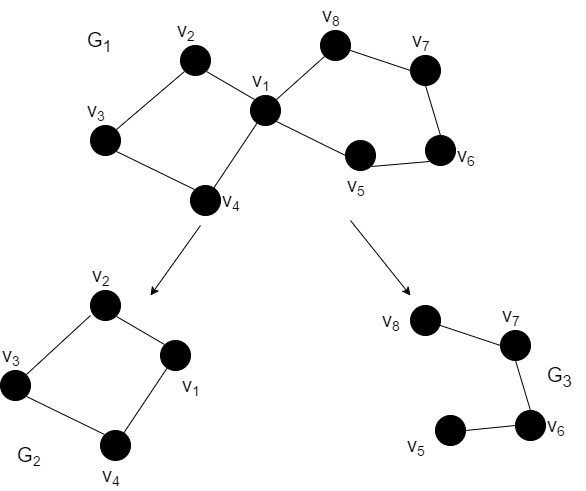
\includegraphics[width=0.7\textwidth]{partition}
\caption{An example of a partition process using edge separator}
\end{figure}

We can see that each time we make a partitioning on a graph, it splits its vertex set and parts of edges set, and removes some edges. if we perform this partitioning recursively until only one vertex left, then we have an edge separator tree from the graph, one edge separator tree for the $G1$ in Figure 2.1 is shown in Figure 2.2. Each vertex in a graph will appear once in a leaf of the edge separator tree build from that graph. Each internal node is the set of edges used as edge separators to make partitioning in each step.

\begin{figure}[h]
\centering
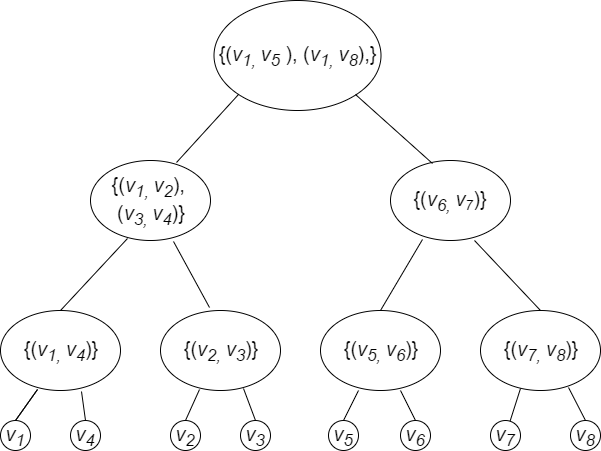
\includegraphics[width=0.8\textwidth]{separatorTree}
\caption{An example of edge separator tree}
\end{figure}


Note that we arbitrarily decide which side of partition will be the left child or the right child in this stage. The tree is also not perfect balanced in some cases (e.g. one child is a leaf and the other is an internal node), the side of the children is also decided arbitrarily. We will take advantages of this "freedom" to further reduce the space to encode the graph in later time. The vertex labels may be disordered by making in-order traversal on the edge separator tree (e.g. in Figure 2.2 the order of the vertexes after in-order traversal is :$v_{1}$, $v_{4}$, $v_{2}$, $v_{3}$, $v_{5}$, $v_{6}$, $v_{7}$, $v_{8}$), we will renumber these vertex by making a in-order traversal along the edge separator tree.


METIS Partition library. To recursively partition the graph, we used METIS's API
in our project. METIS is an open source library developed by Karypis lib in University
of Minnesota. It supports set of serial programs for partitioning graphs and partitioning
nite element meshes. The algorithms implemented in METIS are based on the multilevel
recursive-bisection, multilevel k-way, and multi-constraint partitioning schemes [2]. The
METIS partitioning API returns one integer list with vertex index as key,as well as 0 or 1
as value to indicate which side of partitioning the vertex belongs to (we put the vertexes
with value 0 into left child and vertexes with value 1 into right child). The returned value


\chapter{Index Structure}
\chapter{Conclusion}

Did it!

\bibliographystyle{plain}
\bibliography{bib}

\end{document}
